\documentclass[a11paper, 11pt]{article}

\usepackage{libs/document}
\usepackage{libs/titlepage}
% Allows to include standalone files as figures
\usepackage{graphicx}
\usepackage{float}
\usepackage{standalone}
\usepackage{pgf-umlcd}
\usetikzlibrary{arrows.meta}
\usepackage[T1]{fontenc}
\usepackage[french]{babel}
\usepackage{csquotes}
\usepackage{booktabs}
\usepackage{longtable}
\usepackage{ltablex}
\usepackage{xcolor}

\renewcommand{\umltextcolor}{black}
\renewcommand{\umldrawcolor}{teal}
\renewcommand{\umlfillcolor}{white}

% \addbibresource{bibliography.bib}
% \nofiles

% Petites commandes utiles pour prendres des notes assez visibles
% pour être enlevées facilement
\newcommand{\note}[1]{\textbf{\textcolor{orange}{Note: #1}}}
\newcommand{\todo}[1]{\textbf{\textcolor{teal}{TODO: #1}}}
\newcommand{\fixme}[1]{\textbf{\textcolor{red}{FIXME: #1}}}

% \institution{Université de Sherbrooke}
% \faculty{Faculté de génie}
% \department{Département de génie électrique et de génie informatique}
\title{Rapport d'APP}
\classnb{GIF350}
\class{APP1 -- Modèles de conception}
\author{
  \addtolength{\tabcolsep}{-0.4em}
  \begin{tabular}{rcl} % Ajouter des auteurs au besoin
  Samuel Bilodeau  & -- & BILS2704 \\ % TODO: demander le CIP
  Benjamin Chausse & -- & CHAB1704 \\
  \end{tabular}
}
\teacher{Domingo Palao Munoz}
% \location{Sherbrooke}
% \date{\today}

\begin{document}
\maketitle
\newpage
\tableofcontents
\newpage
\section{Diagrammes de classes de \textit{MenuFact02}}

\begin{figure}[H]
  \centering
	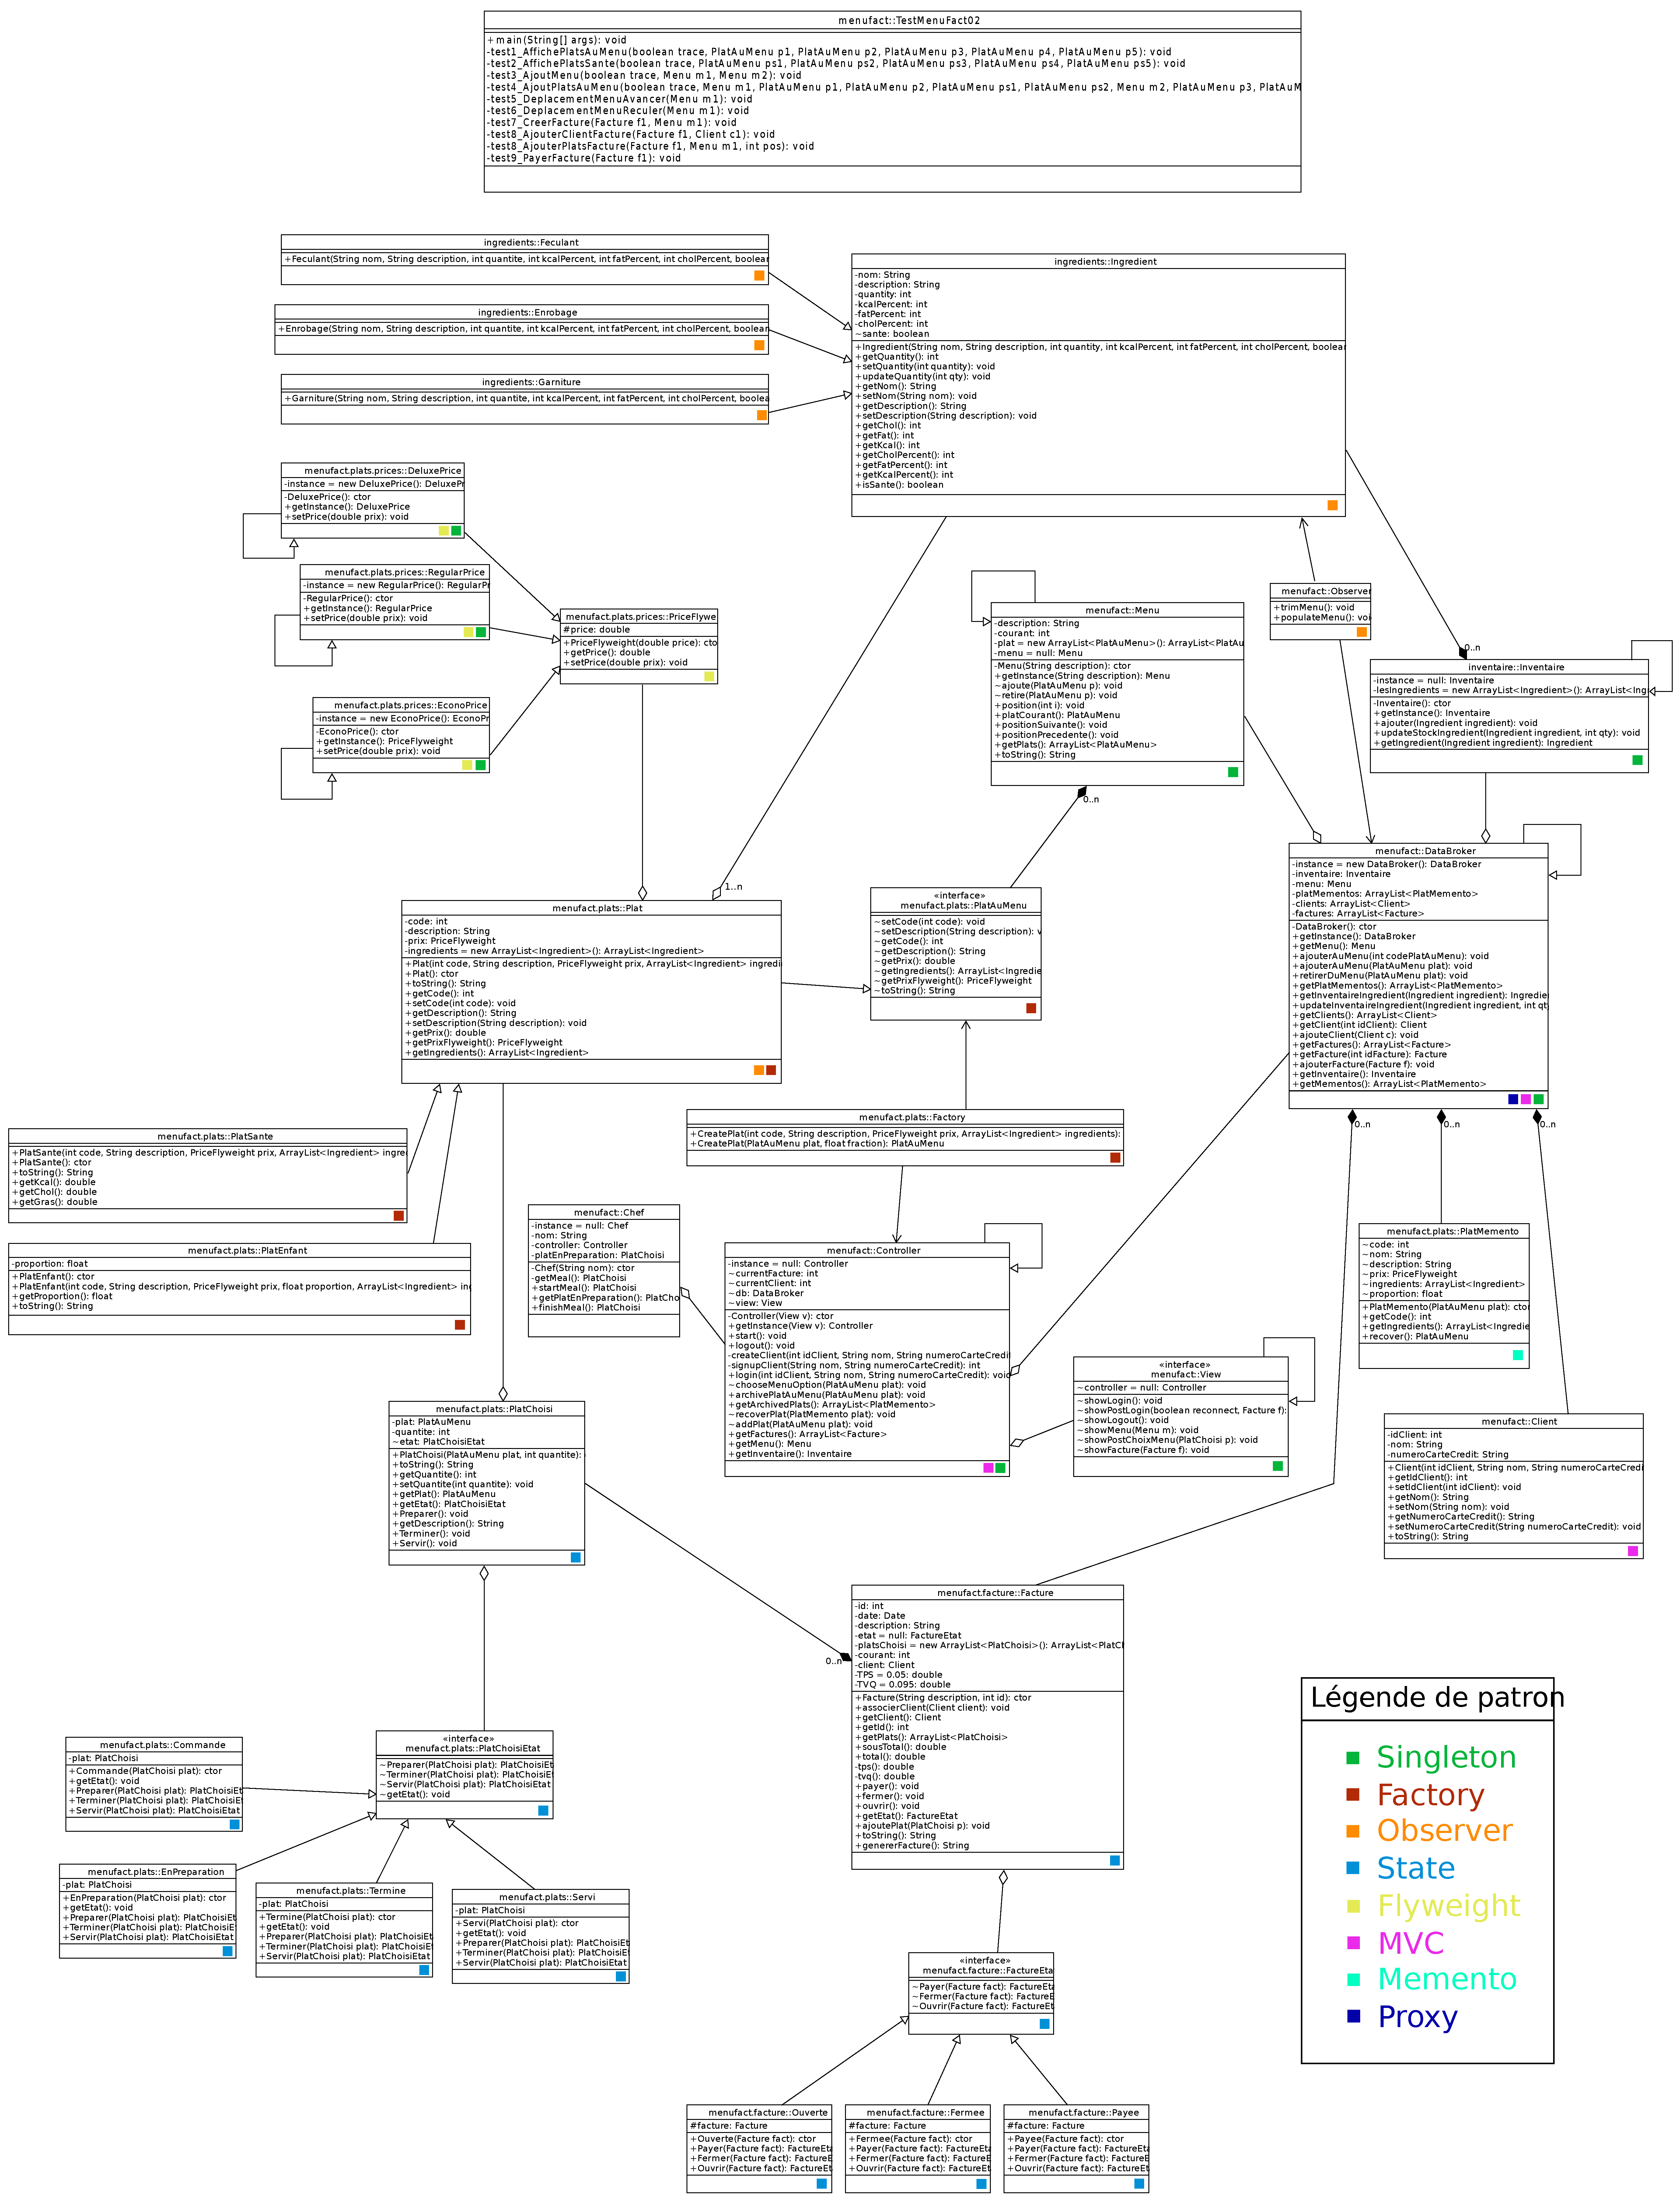
\includegraphics[width=.9\linewidth]{uml/uml.pdf}
  \caption{Diagramme de classes}
  \label{fig:uml}
\end{figure}

\section{Choix de conception}

\begin{table}[H]
\caption{Justification des modèles de conception}
\begin{longtable}{lp{10cm}}
\toprule
\textbf{Modèle de conception} & \textbf{Justification} \\

\midrule
Modèle-vue-contrôleur (MVC) &
Permet de séparer la logique de l'application, l'interface, et l'information
stockée par l'application. \verb|View| est une classe abstraite (qui peut
implémenter une interface web, graphique, terminal, etc\ldots sans changer la
logique) , \verb|Controller| est le cerveau de l'application où la logique
réside et \verb|DataBroker| est le modèle qui stoque les informations de Menu,
factures, Clients, etc\ldots \\

\midrule

Flyweight &
Permet de réduire la mémoire utilisée par l'application en partageant le prix
de tous les plats d'une même gamme de prix. (voir section 2.1) \\

\midrule
States &
Permet de gérer l'état des factures. Une facture peut être dans l'état Ouverte,
Fermée ou Annulée. L'état détermine les actions possibles. Par exemple, il est
impossible d'ajouter des plats à une facture fermée. Il a également été
implémenté pour suivre la préparation des plats entre : commandé, en
préparation, terminé et servi.\\

\midrule
Observer &
La classe \verb|IngredientWatcher| permet de notifier les classes qui s'y
abonnent à chaque fois que les quantités de divers ingrédients passent sous un
seuil critique. Par exemple, le \verb|Controller| pourrait s'abonner à cette
classe pour retirer du menu les plats qui ne peuvent plus être préparés. \\

\midrule
Factory&
La classe \verb|PlatFactory| permet de créer dynamiquement le bon type de plat
selon les ingrédients qu'il contient. Si tous les ingrédients sont santé, un
\verb|PlatSante| sera créé. Sinon ce sera un \verb|Plat| régulier. On peut par
la suite utiliser un plat, santé ou non pour générer un \verb|PlatEnfant| en
lui fournissant un facteur de proportion. Les propriétés nutritives et
caloriques sont storés dans les ingrédients et sont indépendants des plats.\\

\midrule
\end{longtable}
\end{table}
\newpage
\begin{table}[H]
\begin{longtable}{lp{10cm}}

\midrule
Singleton&
Diverses classes sont implémentées en tant que \verb|Singleton| pour éviter
divers problèmes de conception. Par exemple, il n'y a qu'un seul \verb|Menu| et
\verb|Inventaire| pour tout le restaurant (deux clients ne devraient pas avoir
deux menus différents). Il n'y a qu'un seul \verb|DataBroker| pour gérer les
données globales de l'application. On ne veut pas avoir deux bases de données
différentes pour l'application. Finalement il n'y a qu'un seul
\verb|Controller| pour gérer l'application. On veut éviter des problèmes de
synchronisation où deux contrôleurs modifient la même information
simultanément. Cela n'empêche pas l'application d'avoir plusieurs
\verb|View|s qui sont en communication avec le même \verb|Controller|. \\

\midrule Memento&
L'utilisation d'un \verb|Memento| nous a permis de retirer un plat du menu sans
le détruire dès que les ingrédients sont insuffisants à sa conception. Par la
suite, l'\verb|Observer| regarde lorsque les l'inventaires sont ajustés et
retourne chercher en mémoire les plats faisables pour les remettre dans le menu
dynamiquement.\\

\midrule
Proxy&
La classe \verb|Databroker| agit en tant que \verb|Proxy| pour limiter et
réguler les demandes vers les bases de données d'inventaire et de menu.
Plusieurs utilisateurs peuvent être connectés et leur accès contrôlé via cette
porte commune à tous.\\

\bottomrule
\end{longtable}
\end{table}

\subsection{Note sur l'utilisation du \textit{Flyweight}}
\label{flyweight-notes}

Comme mentionné lors du tutorat, l'utilisation de patrons de conception était
surchargée pour le projet. On nous a demandé de les implémenter principalement à
des fins éducationnelles. Ceci dit, pour implémenter le patron
\textit{Flyweight}, nous avons pensé à l'idée d'un restaurant dans lequel les
Plats sont regroupés par gammes de prix (écono, régulier, deluxe). Ainsi,
chaque gamme de prix détient un \textit{flyweights} contenant le prix unique de
tous les plats dans cette gamme. Une économie de mémoire est donc réalisée
puisque la valeur du prix n'est pas dupliquée pour chaque plat d'une même
gamme. Bien sûr, une implémentation réaliste de ce patron contiendrait
généralement plus qu'un seul attribut dans le \textit{flyweights}. Ces classes
seraient donc nommées comme suit:

\begin{itemize}
  \item \verb|Flyweight|: Classe abstraite
  \item \verb|EconoFlyweight|: Classe concrète
  \item \verb|RegularFlyweight|: Classe concrète
  \item \verb|DeluxeFlyweight|: Classe concrète
\end{itemize}

\section{Utilité des modèles de conception}

L'utilisation des modèles de conception comporte plusieurs avantages dans notre application. D'abord, une meilleure organisation du code en divisant les fonctionnalités en plusieurs responsabilités simples, facilitant ainsi la maintenance future. Ensuite, comme les parties du code sont ségréguées entre-elles, il est facile de remplacer ou modifier une section sans impacter tout le reste du code, rendant celui-ci plus évolutif. Sans oublier l'amélioration de la qualité et la réduction de la complexité en général. Le fait d'avoir des structures préétablies certifiées nous a grandement aidés pour aborder les défis de conception de Menufact. Nous recommandons l'utilisation de ceux-ci dans le développement applicatif, mais avec une limite en fonction de l'exhaustivité de ce dernier. En effet, trop de modèles de conception dans une petite application a comme résultat d'augmenter la complexité et par de fait même les possibilités d'erreur donc à utiliser avec modération.\\

\section{Utilité des tests unitaires}

Bien que longs à concevoir, les tests unitaires aident le développement, l'amélioration et la maintenance d'une application. Considérant que ceux-ci se feront tout au long de la durée de vie de l'application, il est très avantageux de les implémenter au début de la conception. Lors de l'ajout d'une fonctionnalité, les tests indiqueront immédiatement si une fonctionnalité fait défaillance ailleurs dans le code à la suite du changement fait. Une fois la batterie de test déployé, le code implémenté devra automatiquement passer cette étape avant d'être fusionné au corps principal du programme éliminant ainsi le risque de nuire à d'autres développeurs. Cette méthodologie a favorisé notre collaboration, aucun code non fonctionnel n'a été partagé. Le résultat attendu devait toujours correspondre, peu importe le changement interne, la sortie restait identique. Cette méthodologie permet de aux développeurs de changer la partie interne d'une application sans impacter l'utilisateur qui ne voie aucune différence. Notre vison du développement applicatif inclura désormais les tests dès le début, car ils augmentent significativement l'efficacité à long terme d'un projet.\\

\newpage
\section{Conclusion}
Pour conclure, nous avons appris à implémenter des patrons de conception et ceux-ci s'avèreront très utiles dans la conception d'applications. Avant de commencer à coder, il faut prendre le temps de voir l'interaction entre les composantes. Repérer si un patron qui pourrait simplifier notre implémentation ou maintenance future, car rappelons-nous que cette dernière sera sans doute plus longue que la conception elle-même. Les tests unitaires sont aussi très importants pour ajouter de la robustesse et faciliter la coopération entre les développeurs. Le tout en accord avec les principes de programmation SOLID qui sont une référence des bonnes pratiques en programmation.\\
% \newpage
% \printbibliography[heading=bibintoc]
\end{document}
